\documentclass[a4paper]{article}
\usepackage{graphicx}
\title{Project Proposal \\ TeX Development Fund}
\author{Keiran Harcombe}
\date{October 2022}
\begin{document}
\maketitle
\section{Project Background} % Describe how this project came about, who is involved and the purpose
Micropress Inc. published an informal math font loosely based on Adobe Tekton. Since the company has gone out of business, an equivalent doesn't exist. You could of course use similar fonts such as Adobe Tekton and P22 Eaglefeather but, to purchase a license for this font would cost around \$380.00 USD. \\
My aim with this project is to create an architectural style font. 

\section{Project Scope} % Project scope defines the boundaries of a project. Think of the scope as an imaginary box that will enclose all the project elements/activities. It not only defines what you are doing (what goes into the box), but it sets limits for what will not be done as part of the project (what doesn’t fit in the box). Scope answers questions including what will be done, what won’t be done, and what the result will look like. 
Utilising support from the scheme
\pagebreak

\section{Research for fonts with similar use cases}
    \begin{figure}[h]
        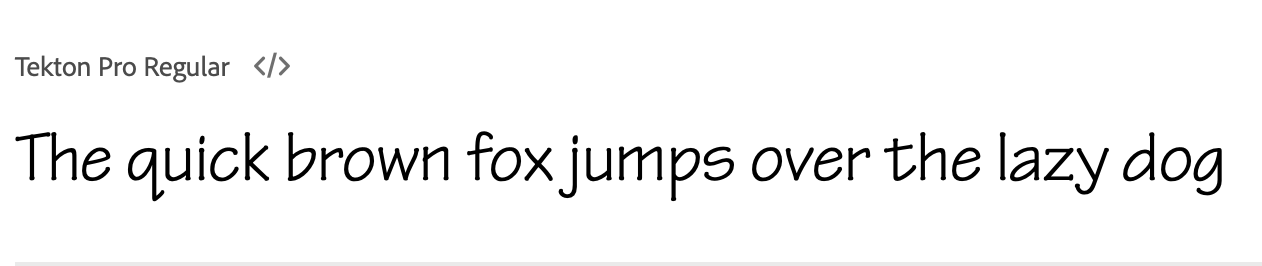
\includegraphics[width=1\textwidth]{Tekton.png}
        \caption{Tekton Pro designed by David Siegel\cite{tekton}}
        \label{fig:tekton}
    \end{figure}
    
    \begin{figure}[h]
        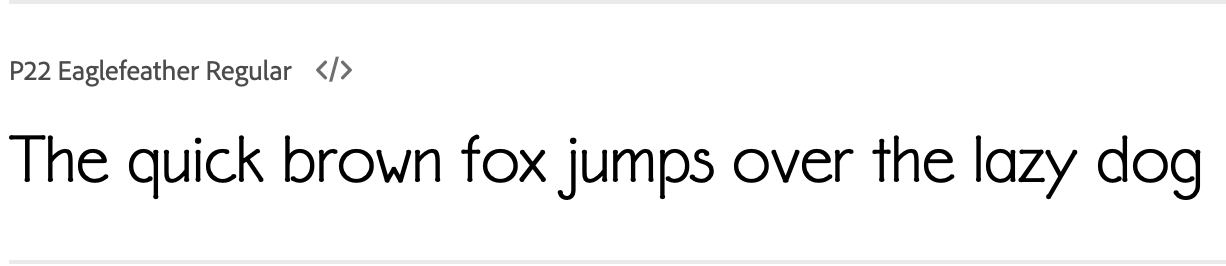
\includegraphics[width=1\textwidth]{Eaglefeather.png}
        \caption{P22 Eaglefeather designed by David Siegel and Frank Lloyd Wright\cite{eaglefeather}}
        \label{fig:eaglefeather}
    \end{figure}

    \begin{figure}[h]
            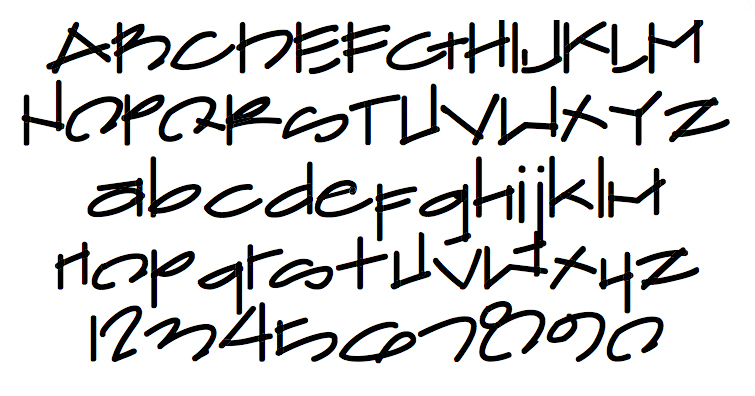
\includegraphics[width=1\textwidth]{ArchitectsFont.jpg}
            \caption{How to Architect Font designed by Doug Patt}
        \label{fig:architects}
    \end{figure}
    
    \begin{figure}[h]
    	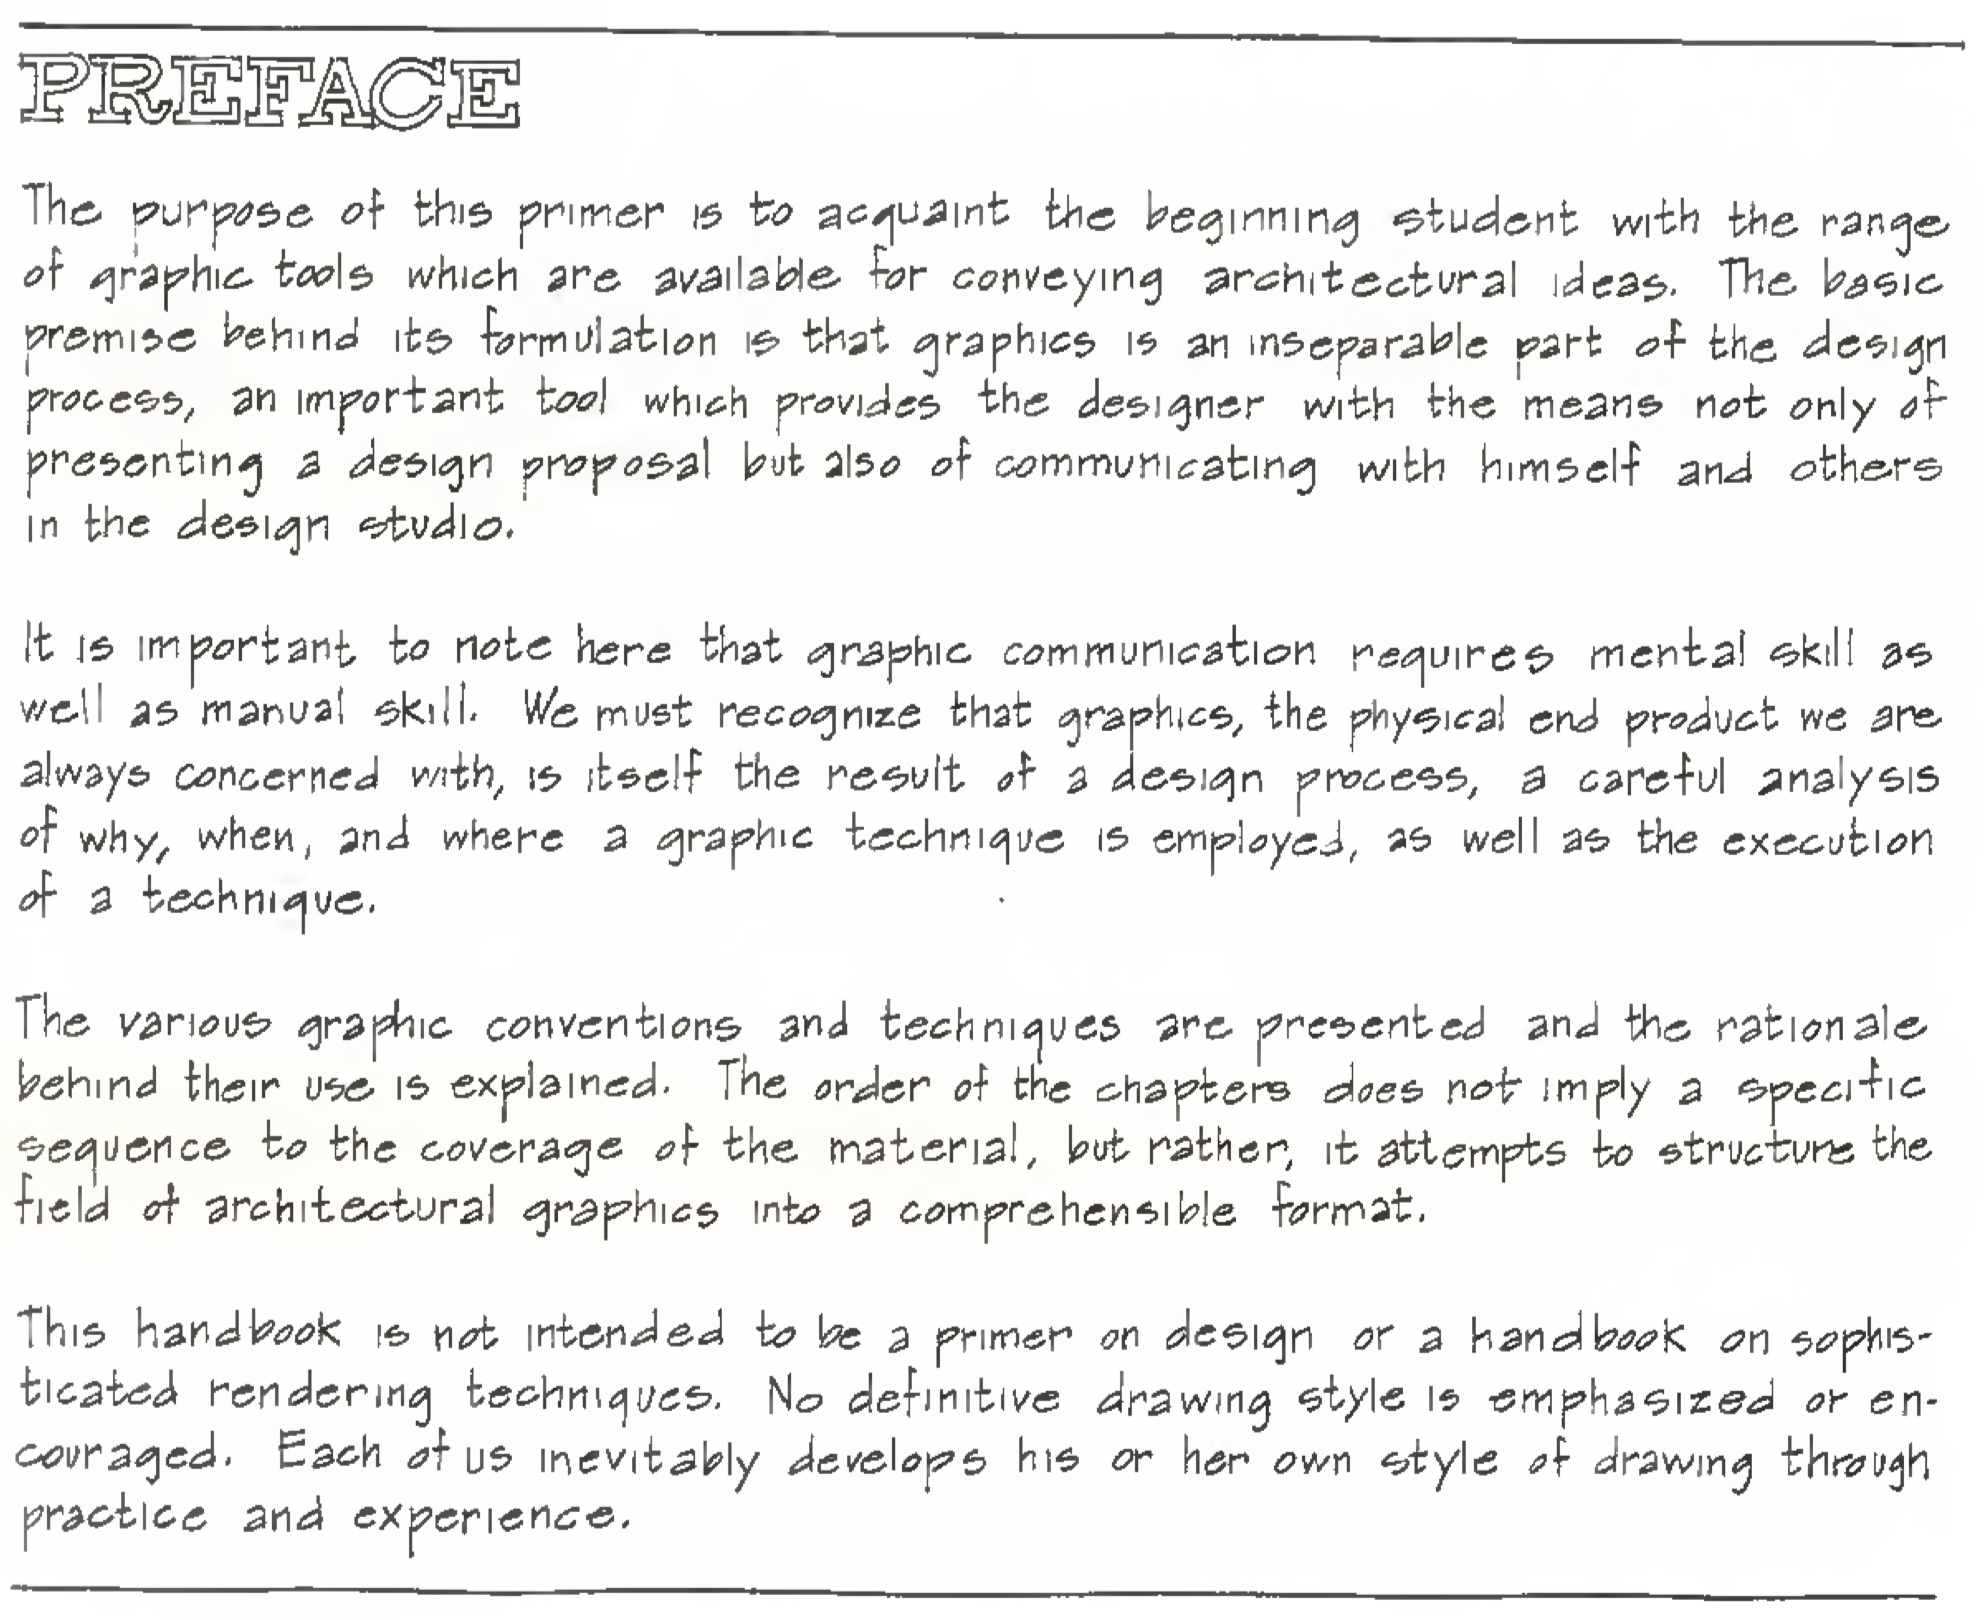
\includegraphics[width=1\textwidth]{Ching.png}
    	\caption{Exerpt from Architectural Graphics\cite{architecturalgraphics}}
    \end{figure}
\pagebreak 
\section{High-Level Requirements} % Describe the high level requirements for the project
Through evaluating similar fonts :
\begin{itemize}
    \item Ability to allow both internal and external users to access the application without downloading any software 
    \item Ability to interface with the existing data warehouse application 
    \item Ability to incorporate automated routing and notifications based on business rules
\end{itemize}

\section{Project Risks}
As with all projects, there is a moderate level of risk. Namely this applies to the announcement by Adobe discontinuing PostScript type 1 fonts. In an attempt to mitigate this risk, the font will be created using the OpenType technology. 
\section{Deliverables} % List agencies, stakeholders or divisions which will be impacted by this project and describe how they will be affected by the project

\section{Affected Parties} % List business processes or systems which will be impacted by this project and describe how they will be affected.

\section{Affected Business Processes or Systems} % Describe any specific components that are excluded from this project.

\section{Specific Exclusions from Scope} % Describe how you plan to implement the project. For example, will all parts of the project be rolled out at once or will it be incremental? What will be included in each release?

\section{Implementation Plan} % Include recommendations that lead to your proposed solution. Summarise what you’re proposing to do and how you’re going to meet the goals. You’ll be able to expand on the details within the ‘Our Proposal’ section.

\section{High-Level Timeline \& Schedule} % List business processes or systems which will be impacted by this project and describe how they will be affected.

\bibliography{bib.bib}
\bibliographystyle{plain}
\end{document}